\section{Data}
\subsection{Genotypes}

The genotypes were processed as described in section~\ref{sssec:gentoypes}. 


\subsection{Phenotypes}
Cardiac magnetic resonance (CMR) images were conducted at Hammersmith Hospital, London. The fractal dimensions are derived from standard 2D CMR images. Scout images were obtained and used to plan 2D cine balanced steady-state free precession images in the left ventricular short axis (LVSA) plane from base to apex. Each section had a thickness of 8 mm with a 2 mm gap between sections. On average 10 to 12 images were recorded per individual \citep{DeMarvao2014}. Fractal analyses was automised according to the processing pipeline proposed by Captur and colleagues \citeyearpar{Captur2013}. In brief, the images were binarised into blood pool and myocard and the endomyocardial border was extracted via edge detection. The FD was determined by placing grids with known spacing (scale) of increasing size (i.e. increasing number of edges) on the image and counting the number of boxes with non-zero pixels, i.e. how many boxes contain at least one pixel of border. The slope of the linear regression of the log transformed scale versus the log transformed counts corresponds to the FD \citep{Captur2013}.

\begin{figure}[hbtp]
	\centering
	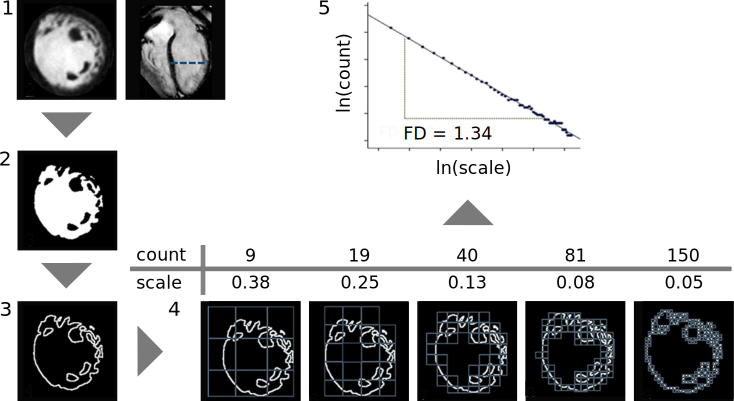
\includegraphics[trim = 0mm 0mm 0mm 0mm, clip, width=\textwidth]{Chapter5/Figures/FD_scheme.pdf}
	\caption{\textbf{.}.} 
	 	\label{fig:FD}
\end{figure}